\section{Metodologia}
No desenvolvimento desta pesquisa foram utilizados modelos de machine learning na tentativa de se obter material comparativo entre métodos mais tradicionais de modelagem e uma rede neural bayesiana.

O Conjunto de dados é fictício, mas serve como motivação para futuras pesquisas com dados reais acerca deste tema, de fato o entendimento do que define um bom desempenho escolar é um tema que não deve ser negligênciado por aqueles que visão melhorar a educação como um todo.




\subsection{Os dados}

Os dados foram obtidos a partir do site kaggle\cite{kaggle} e são fictícios, apesar disso ainda são muito úteis para que possamos ter ideias de possíveis análises e abordagens acerca do tema. A base de dados conta com 15 colunas onde uma é um índice, 9 são categóricas e 5são núméricas, destas 5, 3 são variáveis resposta, scores divididos entre leitura, escrita e matemática.

A tabela 1 a seguir resume sobre o que cada variável significa.\\

\begin{table}[htbp]
    \centering
    \caption{Descrição das Variáveis}
    \begin{tabular}{|c|p{8cm}|}
        \hline
        \textbf{Variável} & \textbf{Descrição} \\
        \hline
        Gender & Gênero do estudante \\
        \hline
        EthnicGroup & Grupo Étnico do estudante, de A a E \\
        \hline
        ParentEduc & Nível de escolaridade dos pais \\
        \hline
        LunchType & Tipo de merenda escolar (padrão ou gratuita/reduzida) \\
        \hline
        TestPrep & Teste preparatório, completo ou não \\
        \hline
        ParentMaritalStatus & Status civil dos pais \\
        \hline
        PracticeSport & Freqência com que pratica esportes \\
        \hline
        IsFirstChild & Se é ou não primeiro filho \\
        \hline
        NrSiblings & Número de irmãos do estudante \\
        \hline
        TransportMeans & Meio de locomoção para a escola \\
        \hline
        WklyStudyHours & Horas semanais de estudo, menos de 5 horas; entre 5 e 10 horas; mais de 10 horas \\
        \hline
        MathScore & Score de matemática\\
        \hline
        ReadingScore & Score de leitura \\
        \hline
        WritingScore & Score de escrita \\
        \hline
    \end{tabular}
    \label{tab:variaveis}
\end{table}

\newpage
\subsection{Árvore de decisão}

O primeiro modelo ajustado para ser usado como comparativo foi uma árvore de decisão, árvores são modelos hierárquicos, isto é, modelos que usam uma série de perguntas para levar a uma decisão, estas perguntas são criadas observando um número grande de outras amostras do mesmo problema\cite{arvore}.

A árvore é formada por nós, ramos e nós folhas, onde cada nó divide a árvore baseado em um atributo do conjunto de dados, cada ramo é a representação dos valores que estão classificados em cada nó e os nós folhas ou final representam o fim da árvore onde os dados estão separados após passarem por todos os nós.

\begin{figure}[htbp]
  \centering
  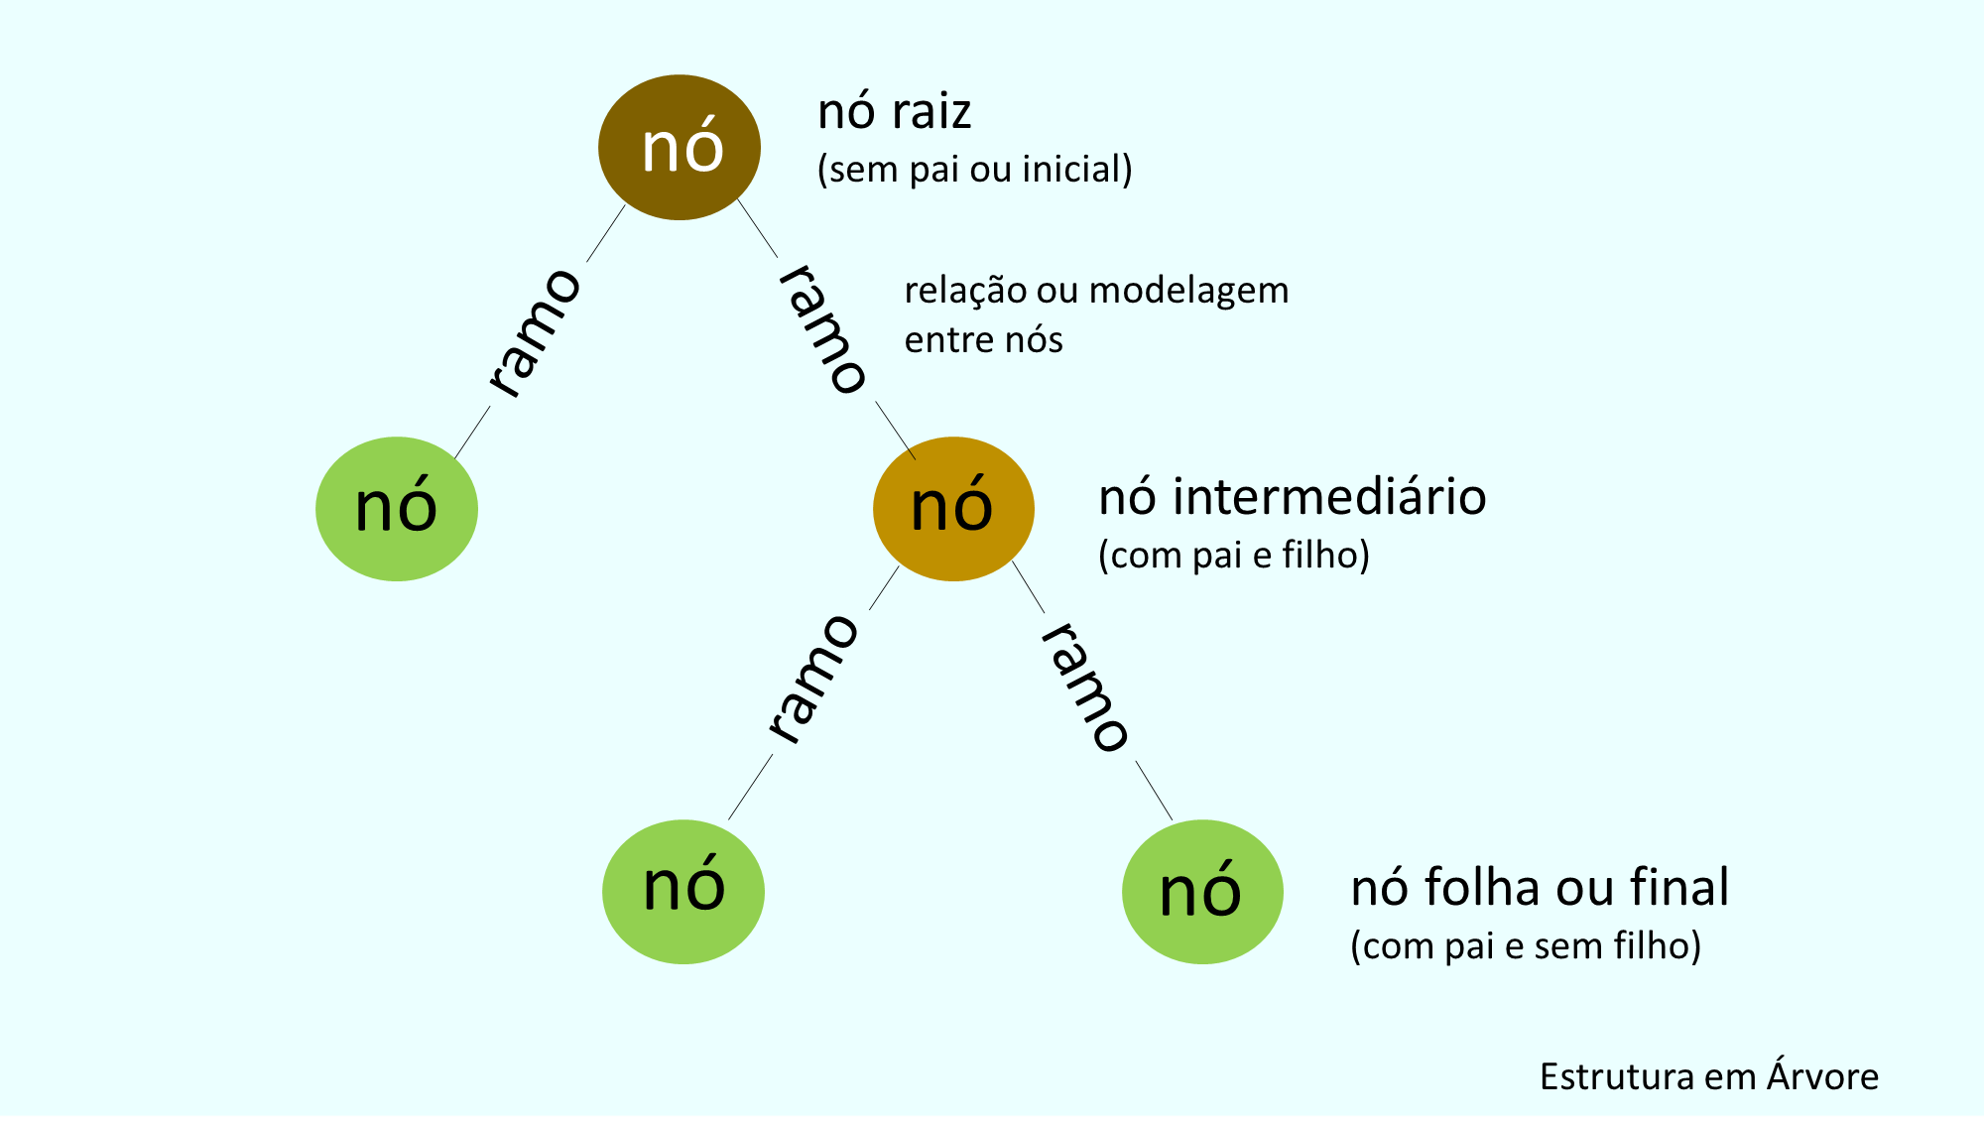
\includegraphics[width=0.8\textwidth]{arvore.png}
  \caption{Exemplo de árvore de decisão} {\footnotesize Fonte: \href{https://colaborae.com.br/blog/2023/07/19/arvore-de-decisao/}{Colaborae}}
  \label{fig:exemplo}
\end{figure}


Para decidir qual o melhor ponto de corte de uma variável e o quanto essa variável traz de ganho para separar a informação, usou-se o critério do erro quadrático médio (MSE). O MSE é calculado como a média dos quadrados das diferenças entre os valores previstos e os valores reais. O objetivo do modelo é minimizar o MSE durante o processo de treinamento, o que significa que ele busca encontrar a árvore de decisão que melhor se ajusta aos dados de treinamento, minimizando o erro médio ao prever os valores alvo.

\subsection{Floresta aleatória}


Uma floresta aleatória (Random Forest) é um tipo de algoritmo de aprendizado de máquina que é usado tanto para tarefas de classificação quanto para regressão. É uma técnica de conjunto (ensemble) que combina várias árvores de decisão individuais para criar um modelo mais robusto e preciso.

A ideia fundamental por trás da floresta aleatória é criar várias árvores de decisão independentes durante o processo de treinamento. Cada árvore de decisão é treinada em uma amostra aleatória dos dados de treinamento e, durante a construção da árvore, em cada divisão de nó, apenas um subconjunto aleatório das características (variáveis) é considerado para determinar a melhor divisão. Isso introduz aleatoriedade e diversidade no processo de construção das árvores\cite{riqueti2018classificando}.

Após treinar todas as árvores de decisão, a previsão de uma nova instância é feita pela maioria das previsões das árvores individuais no caso de classificação (voto majoritário) ou pela média das previsões no caso de regressão.

\begin{figure}[htbp]
  \centering
  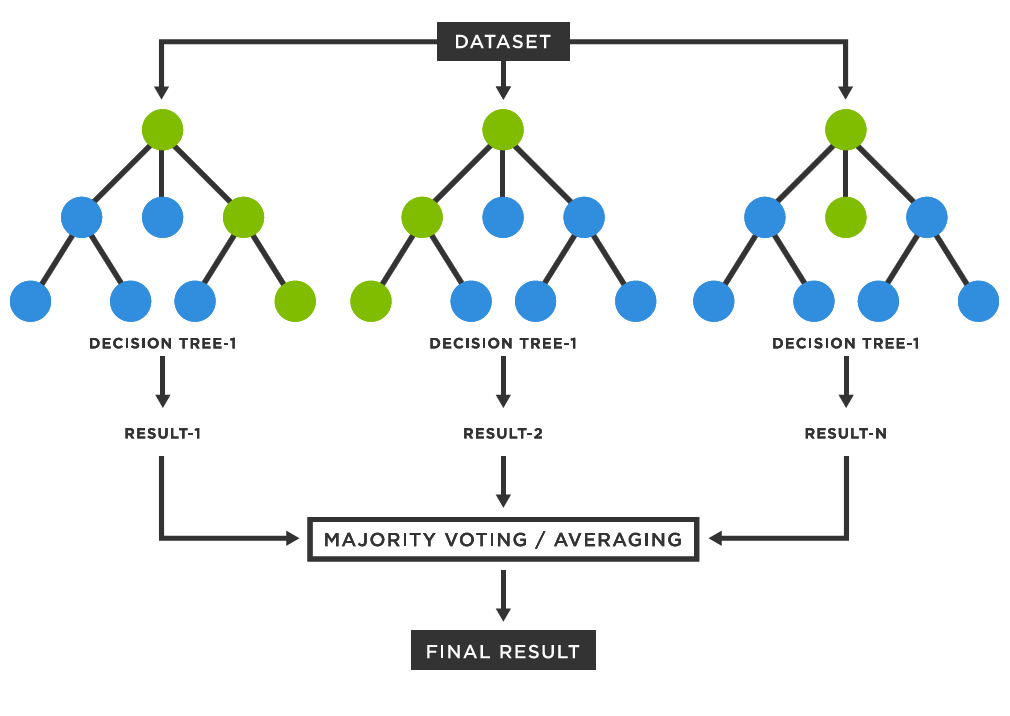
\includegraphics[width=0.8\textwidth]{Floresta.png}
  \caption{Exemplo de Floresta aleatória} {\footnotesize Fonte: \href{https://medium.com/@denizgunay/random-forest-af5bde5d7e1e}{Deniz Gunay}}
  \label{fig:Floresta aleatória}
\end{figure}

\section{Rede neural}

A rede neural tem como objetivo tentar simular a maneira como um cérebro humano pensa, criando neurônios e fazendo ligações entre eles, o conceito de rede neural surgiu com o modelo matemático de um neurônio biológico proposto por Warren McCulloch e Walter Pitts
em 1943. O modelo, denominado neurônio MCP (McCulloch-Pitts), é descrito por um conjunto de n entradas, as quais são multiplicadas por um determinado peso e, em seguida, os resultados são somados e comparados a um limiar\cite{fleck2016redes}.

Atualmente existem diversos modelos de redes neurais, cada um mais adequado para a resolução de um problema específico, a seguir alguns dos principais modelos de redes neurais

\begin{itemize}
    \item \textbf{Feedforward Neural Networks (Redes Neurais de Avanço)}:
    Também conhecidas como redes neurais multicamadas (Multilayer Perceptrons - MLPs), essas redes consistem em uma sequência de camadas de neurônios, onde as conexões entre os neurônios não formam ciclos. Essas redes são usadas para tarefas de classificação, regressão e outras, dependendo da arquitetura específica\cite{enwiki:1216115889};
    
    \item \textbf{Convolutional Neural Networks (Redes Neurais Convolucionais - CNNs)}:
    Essas redes são projetadas para processar dados de grade, como imagens. Elas usam camadas de convolução para aprender características espaciais, reduzindo a quantidade de parâmetros e melhorando a eficiência do aprendizado em dados de imagem. As CNNs são amplamente usadas em tarefas de visão computacional, como reconhecimento de imagem, segmentação e detecção de objetos\cite{gu2018recent};
    
    \item \textbf{Recurrent Neural Networks (Redes Neurais Recorrentes - RNNs)}:
    Essas redes são projetadas para processar sequências de dados, onde as conexões entre neurônios formam loops, permitindo que a rede mantenha uma memória de estados anteriores. As RNNs são usadas em tarefas como processamento de linguagem natural (NLP), tradução de idiomas, previsão de séries temporais e muito mais\cite{RNN};
    
    \item \textbf{Generative Adversarial Networks (Redes Generativas Adversariais - GANs)}:
    Este tipo de rede neural consiste em duas redes neurais, um gerador e um discriminador, que são treinadas simultaneamente em uma competição entre si. As GANs são usadas para gerar dados novos e realistas, como imagens, áudio e texto\cite{wang2017generative}.
\end{itemize}

Para o presente trabalho, foi aplicada uma rede neural feedfoward, por ser mais indicada para lidar com casas de regressão, trabalhou-se com uma rede neural com 2 camadas, sendo a primeira com 3 neurônios com ativação ReLU e a segunda a camada de saída linear

A ativação ReLU (Rectified Linear Unit) é definida como:

\begin{center}
\centering
$f(x) = \max(0, x)$
\end{center}

A principal razão para o uso da função ReLU é a sua simplicidade computacional e eficácia em redes neurais profundas. Algumas das suas características incluem:

\begin{itemize}
    \item \textbf{Não saturação}:
    A função ReLU não satura para valores positivos de entrada, o que significa que ela não fica presa em uma faixa de valores onde a derivada é zero durante o treinamento, como acontece com funções de ativação como a sigmoide e a tangente hiperbólica. Isso ajuda na prevenção do desaparecimento do gradiente, tornando o treinamento mais rápido e eficiente;
    
    \item \textbf{Esparsidade de ativação}:
    A função ReLU induz uma esparsidade nas ativações da rede, o que significa que menos neurônios são ativados, resultando em redes mais eficientes computacionalmente;
    
    \item \textbf{Facilidade de interpretação}:
    A função ReLU torna as previsões do modelo mais fáceis de interpretar, pois os valores de saída positivos são diretamente proporcionais às entradas positivas, o que facilita a compreensão do comportamento do modelo.
\end{itemize}

\section{Rede neural Bayesiana}

Os procedimentos tradicionais para determinar os parâmetros das redes neurais vem a partir da aplicação dos princípios estatísticos de máxima verossimilhança. No entanto, essas técnicas podem apresentar diversas limitações. Por contraste, a utilização de métodos estatísticos Bayesianos na estimativa dos parâmetros oferece a vantagem de modelar tais relações com base em distribuições probabilísticas. Isso possibilita a realização de aproximações das funções enquanto se considera a estimativa de suas incertezas.\cite{rodriguezrede}

Nas redes neurais Bayesianas, o objetivo é construir a função de distribuição de
probabilidade a posteriori dos parâmetros da rede, com base nos dados disponíveis.
Dessa maneira, densidades de probabilidade são construídas em cada ponto do espaço
de parâmetros da rede.\cite{rodriguezrede}

A abordagem Bayesiana traz várias características importantes, como:
\begin{itemize}
    \item o treinamento convencional baseado na minimização de uma função de erro pode ser
visto como um caso particular do tratamento Bayesiano geral;
    
    \item a abordagem Bayesiana possui de modo natural, uma técnica de regulação de
parâmetros pela qual são penalizados os parâmetros que possuem valores altos;
    
    \item ¾ o método Bayesiano permite que os valores dos coeficientes de regulação sejam
selecionados a partir dos dados de treinamento, desta forma não precisa separar um
conjunto de dados para a validação cruzada;
    
    \item a abordagem Bayesiana permite fazer a comparação de modelos (redes com diferente
número de neurônios da camada escondida), usando só os dados de treinamento
(princípio de Occam’s razor); \cite{Tito1999}
\end{itemize}


